\documentclass{article}

\usepackage[margin=1.6cm]{geometry}
\usepackage{amsmath,amssymb}
\usepackage{float}
\usepackage{graphicx}
\usepackage{fancyhdr}
\pagestyle{fancy}
\usepackage{tcolorbox,listings}
\usepackage{color}
\usepackage{hyperref}
\renewcommand\headrulewidth{1pt}
\usepackage{marvosym}
\usepackage{xcolor}
\usepackage{tikz}
%\usepackage{babel}
\usepackage[french]{babel}
\usepackage[babel=true,kerning=true]{microtype}
\usepackage{afterpage}

\newcommand\myemptypage{
    \null
    \thispagestyle{empty}
    \addtocounter{page}{-1}
    \newpage
    }

\usetikzlibrary{
  arrows,
  calc,
  shapes.geometric,
  shapes.misc,
  shapes.symbols,
  shapes.arrows,
  automata,
  through,
  positioning,
  scopes,
  decorations.shapes,
  decorations.text,
  decorations.pathmorphing,
  shadows}

\definecolor{darkWhite}{rgb}{0.94,0.94,0.94}
 
\lstset{
    backgroundcolor=\color{darkWhite},
    breakatwhitespace=false,
    breaklines=true,
    captionpos=b,
    commentstyle=\color{green},
    deletekeywords={...},
    escapeinside={\%*}{*)},
    extendedchars=true,
    keepspaces=true,
    keywordstyle=\color{blue},
    %language=Python,
    morekeywords={*,...},
    showspaces=false,
    showstringspaces=false,
    showtabs=false,
    stepnumber=1,
    stringstyle=\color{gray},
    tabsize=4,
}
 
\lstdefinestyle{frameStyle}{
    basicstyle=\sffamily,
    numbers=left,
    numbersep=20pt,
    numberstyle=\tiny\color{black}
}
 
\tcbuselibrary{listings,skins,breakable}
 
\newtcblisting{customFrame}{
    arc=0mm,
    top=0mm,
    bottom=0mm,
    left=3mm,
    right=0mm,
    width=\textwidth,
    listing only,
    listing options={style=frameStyle},
    breakable
}

\fancyhead[L]{ALLEMAND Fabien\\COUTURE Louise}
\fancyhead[C]{Modèle de Connaissances\\et Web Sémantique}
\fancyhead[R]{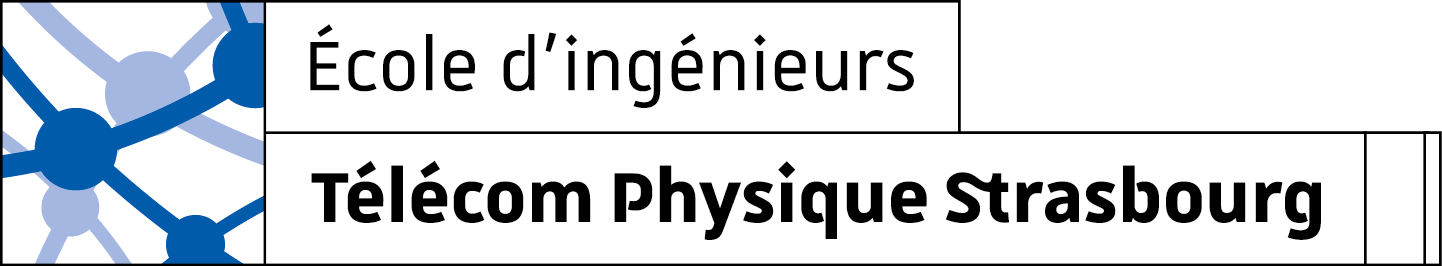
\includegraphics[scale=0.4]{img/logo_TPS_1.png}}
\fancyfoot[L]{Rapport de Projet}
\fancyfoot[R]{\today}

\begin{document}

\thispagestyle{empty}
\addtocounter{page}{-1}
\begin{center}
	\baselineskip=50pt
	\vspace*{1cm}
	\textbf{{\Huge Modèle de Connaissances\\et Web Sémantique}}\\
	\vspace*{0.25cm}
	\textbf{{\Huge Rapport de Projet}}\\
	\vspace*{0.25cm}
	\begin{minipage}[c]{.46\linewidth}
        \centering
        \textbf{Groupe:}\\
		ALLEMAND Fabien\\
        COUTURE Louise
    \end{minipage}
\end{center}
\vspace{0.1cm}

\begin{figure}[H]
\centering
\centerline{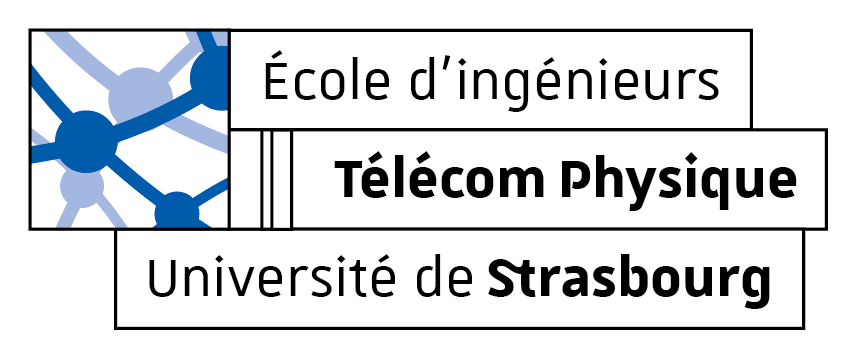
\includegraphics[scale=2]{img/logo_TPS_2.png}}
\end{figure}

\newpage
\section{Construction de l'Ontologie}

L'objectif de ce projet est de créer une ontologie OWL permettant de représenter le plus précisément possible les informations sur des chansons. Pour cela, nous utilisons le logiciel Protégé développé par l'Université de Stanford ainsi que l'ontologie FOAF (Friend Of A Friend) comme base de notre ontologie.\\
Nous avons tout d'abord créé des classes primitives correspondant aux chansons, aux groupes, aux musiciens (et leurs spécialités) et aux récompenses. Puis nous avons ajoutés diverses classes définies pour répondre à nos besoins.

\begin{figure}[H]
    \center
    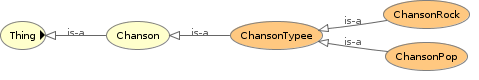
\includegraphics[scale=.5]{img/chanson.png}
    \caption{Hiérarchie des chansons}
\end{figure}

\begin{figure}[H]
    \center
    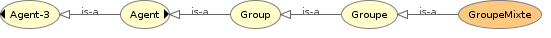
\includegraphics[scale=.5]{img/groupe.png}
    \caption{Hiérarchie des groupes}
\end{figure}

\begin{figure}[H]
    \center
    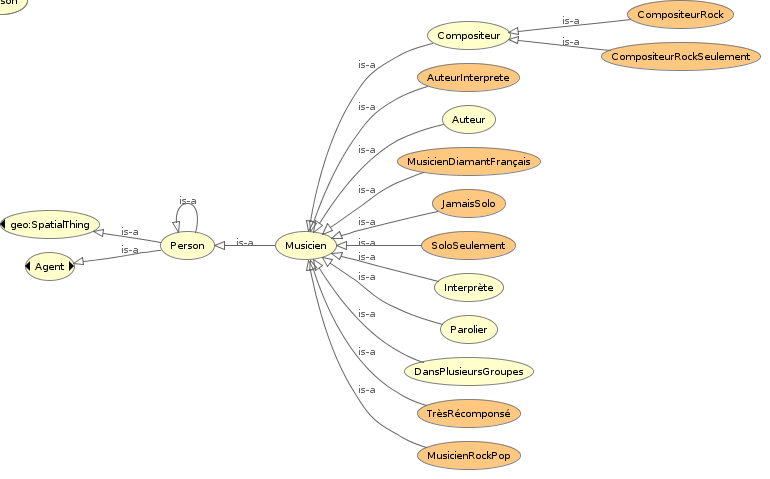
\includegraphics[scale=.5]{img/musicien.png}
    \caption{Hiérarchie des musiciens}
\end{figure}

\begin{figure}[H]
    \center
    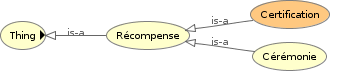
\includegraphics[scale=.5]{img/recompense.png}
    \caption{Hiérarchie des récompenses}
\end{figure}

\newpage
\section{Interrogation de l'Ontologie}

\end{document}